[132 v\textsuperscript{o}] semblables, en tous les autres points assignables. Et par consequent une confusion generalle, laquelle seroit moindre sans doute, si les trois corps \textit{a}, \textit{b}, \textit{c} estoit pr\`{e}s l'un de l'autre dans la situation \textit{a}, \textit{bb}, \textit{cc}. Et comme le mouuement general tache de disposer les corps d'une maniere dont il soit empech\'{e} le moins qu'il est possible (comme je suppose d'estre demontr\'{e} ailleurs) les trois corps donnez se joindront ensemble de cette facon susdite \edtext{ou}{\lemma{susdite}\Afootnote{ \textit{ (1) }\ . Q. E. D. \textit{ (2) }\  et \textit{ (3) }\ ou \textit{ L}}} qui est la même chose, \edtext{prenant l'espace \textit{hegf} pour la region de nostre terre, la nature s'opposera}{\lemma{chose,}\Afootnote{ \textit{ (1) }\ la cho \textit{ (2) }\ la   Nature empechera \textit{ (3) }\ prenant [...] s'opposera \textit{ L}}} \`{a} la \edtext{discontinuation des corps}{\lemma{la}\Afootnote{ \textit{ (1) }\ dissolution des corps \textit{ (2) }\ discontinuation des corps \textit{ L}}} sensibles.
\pend 
%Zeitz auskommentiert    \begin{center}                    
%    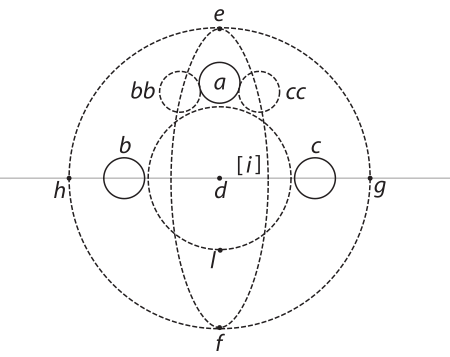
\includegraphics[width=0.5\textwidth]{images/37_3_132r}\\\textit{[Fig. 1]}
%    \end{center}
\pstart L'application de cette proposition aux phenomenes proposez s'\'{e}claircira par la solution des objections principalles.\edlabel{principallesstart}\pend 
\pstart \edtext{\textso{Object. 1.} Il s'ensuiuroit, que deux corps l'un liquide, l'autre solide comme le verre, et l'eau, ne se separeroient pas, même quand\edlabel{principallesend}}{\lemma{principalles.}\xxref{principallesstart}{principallesend}\Afootnote{ \textit{ (1) }\ \textso{Object. 1.} Il s'ensuiuroit, que non seulement les corps demeureroient unis dans le vuide\protect\index{Sachverzeichnis}{vide|textit}, mais a \textit{ (2) }\ \textso{Object.} [...] solide  \textbar\ comme le verre, et l'eau \textit{ erg.}\ \textbar\ , ne [...] quand \textit{ L}}} il y a une bulle d'air entre deux, \textso{contre le phenomene 5.} Car le mouuement general tachera de les joindre autant qu'il est possible, et pressera l'air dans un petit espace, pour estre moins empech\'{e}. La response se tire ais\'{e}ment de nostre proposition. Car cette joinction arrive, s'il n'y a point d'autre remede. Mais dans le cas propos\'{e}, il faut considerer qu'il y a deux efforts de la Nature, ou du mouuement general, l'un, \`{a} joindre les corps heterogenes, grossiers ou sensibles, l'autre \`{a} les dissiper ou dilater \edtext{s'ils sont capables}{\lemma{dilater}\Afootnote{ \textit{ (1) }\ l'air, qui est capable \textit{ (2) }\ s'ils sont capables \textit{ L}}} de dilatation; \edtext{mais comme}{\lemma{dilatation;}\Afootnote{ \textit{ (1) }\ puisque \textit{ (2) }\ comme nous avons  \textit{(a)}\ demontr\'{e} \textit{(b)}\ montr\'{e} \textit{ (3) }\ car nous avons montr\'{e} \textit{ (4) }\ mais comme \textit{ L}}} l'air seul en est capable, ces deux efforts\edtext{}{\lemma{}\Afootnote{efforts  \textbar\ egaux \textit{ erg. u.}\  \textit{ gestr.}\ \textbar\ l'un \textit{ L}}} l'un de dilater l'air, interpos\'{e} (et par consequent (1), de separer les corps) et l'autre de joindre les corps, combattront ensemble, et le premier sera assist\'{e} par la pesanteur de la liqueur, il l'emportera donc sur l'autre, et la liqueur tombera, selon \textso{le phenomene 5.}\pend \pstart \textso{Object. 2.} \edtext{Il s'ensuiuroit}{\lemma{\textso{2.}}\Afootnote{ \textit{ (1) }\ selon \textit{ (2) }\ Il s'ensuiuroit \textit{ L}}} d'avantage que les corps sensibles\protect\index{Sachverzeichnis}{corps!sensible} se deuroient même approcher dans le vuide\protect\index{Sachverzeichnis}{vide} l'un de l'autre, contre l'experience. La Response en est, que cela arriveroit dans un vuide\protect\index{Sachverzeichnis}{vide} parfait pourveu que les corps ne soient pas trop pesans,